\section{New physics models and how to search for them}

%The most pessimistic solution to the flavour problem is Minimal Flavour Violation (MFV)
%which simply assumes that beyond SM physics follows a Yukawa coupling like structure in the flavour
%sector, this would lead to no discernible new physics in the flavour sector.
The most general way to parameterize NP is with an effective Lagrangian describing generic
interactions at an energy scale $\mu$, in which long and short distance effects are separated.
Long distance (equivalently low energy) effects are described by coefficients, $c$, which can be
calculated using perturbative methods.
Short distance (or high energy) effects are characterized by terms of operators, $\mathcal{O}$,
which must be calculated non-perturbatively because they contain QCD interactions.
The resulting effective Lagrangian includes a sum over all processes, $i$, which contribute at a
given dimension, $d$:
\begin{equation}
  \Lag{eff}
  =
  \Lag{SM} + \sum_d\frac1{\Lambda^{d-4}}
  \sum_ic_i^{(d)}\mathcal{O}_i^{(d)}.
  \label{eq:th:lageff}
\end{equation}
Processes that cause FCNCs contribute in $d=6$, and can be written as
\begin{equation}
  \Delta\mathcal{L}^\mathrm{FCNC}
  =
  \sum_{i\neq j}\frac{c_{ij}}{\Lambda^2}
  \left(\Xbar{\mathcal{O}}_{Li}\gamma^\mu\mathcal{O}_{Lj}\right)^2,
\end{equation}
where $c_{ij}$ are dimensionless FCNC couplings, where $i$ and $j$ are different quark generations.
Bounds set on the energy scale $\Lambda$ by the analysis in \Ref{Isidori:2010kg} are:
\begin{equation}
  \Lambda > \frac{|c_{ij}|^\frac12}{|\Vconj{ti}\V{tj}|}\times4.4\tev
  \sim
  \left\{
    \begin{array}{l}
      |c_{sd}|^\frac12\times 1.3\e{4}\tev \\
      |c_{bd}|^\frac12\times 5.1\e{2}\tev \\
      |c_{bs}|^\frac12\times 1.1\e{2}\tev \\
    \end{array}\right.
\end{equation}
These values are calculated under the assumption that NP has a natural flavour structure, where
$c_{ij}\approx\mathcal{O}(1)$.
So, either couplings are of order unity and NP begins to contribute at over $100\tev$; or couplings
strengths are $\mathrm{O}(10^{-5})$ and NP contributes at the $1\tev$ level;
it is expected for NP to appear at the $1\tev$ scale in order to solve the hierarchy problem.
Either way, there is a conflict between the most natural coupling and energy scale; this is known
as the \emph{flavour problem}.
This leads to a host of contradictions, leading to the conclusion that NP has a highly non-generic
flavour structure.

The most pessimistic solution to the flavour problem is Minimal Flavour Violation (MFV)
which simply assumes that beyond SM physics follows a Yukawa coupling like structure in the flavour
sector, this would lead to no discernible new physics in the flavour sector.
Assuming that nature has not chosen MFV, then contradictions from flavour problem indicate that NP
searches should be made for both: particles
with high mass, and particles which have small coupling strengths.
The \lhcb experiment can probe the mass scale, since precision measurements of tree and loop
diagrams are sensitive to virtual particles contributing at all orders, whose on-shell mass could
be many TeV.
The relatively high luminosity of interactions supplied by the \lhc mean that \lhcb is also
sensitive to low coupling strengths, such as messenger particles from the dark sector.
The following chapters explore a variety of different searches for beyond Standard Model physics.

\begin{figure}
  \begin{center}
    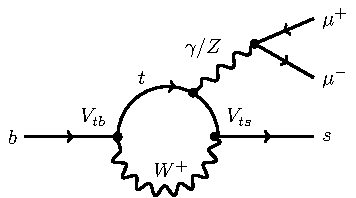
\includegraphics[scale=1]{feynman_btosmumu_penguin}
    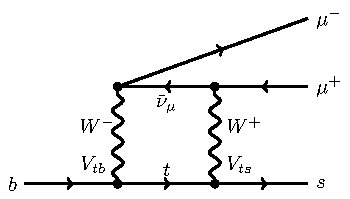
\includegraphics[scale=1]{feynman_btosmumu_box}
    \caption[Schematic Feynman diagrams for loop and box diagrams]
    {\small
      Schematic Feynman diagrams for the
      (left) penguin loop diagrams corresponding to the operators \Op{7} and \Op{9} depending on
      whether a $\gamma$ or $Z$ is emitted from the loop;
      (right) \Op{10} box diagram mediated by \Wp bosons.
    }
    \label{fig:hhh:loops}
  \end{center}
\end{figure}

As well as in loops, virtual particles can also contribute in some tree level diagrams.
The small value of $|\V{ub}|$ means that annihilation decays of \Bp mesons are heavily
suppressed in the SM.
%They are mediated by
%Tree level diagrams in the SM are typically high statistics modes, however annihilation type decays
%are heavily suppressed.
These rare modes are propagated by a \Wp in the SM; but this could be exchanged for any charged
boson, such as an $H^+$ from SUSY, this could alter the branching fraction or
introduce significant \CPV.
%The decay \btodsphi is an annihilation decay of the \Bp.

%New physics models must be able to accommodate Dark Matter.
%Some models have a \emph{dark} or \emph{hidden} sector which, apart from gravity, only
%communicates with the visible sector feebly via messenger particles.
%These messenger particles could potentially be observed after they decay into SM particles after
%mixing with a $H$ or $Z$.
%The axion could be such a particle, as could the inflaton or dark $Z$; models including these
%particles are further detailed in \Sec{sec:db:intro}.
%
%%Dark Matter is the lightest supersymmetric particle which is stable and messenger particle is super
%%goldstino
%Supersymmetry (SUSY) is a theory which introduces an additional super-particle for each SM fermion and
%gauge boson, whose spin is different by a half integer.
%The Higgs sector in SUSY comprises four Higgs doublets; two are spin-0 and two are spin-$\tfrac12$,
%and then there are two each for $Y=\pm\tfrac12$.
%After SUSY is broken there are five Higgs physical scalar particles, two are \CP-even ($h^0$,
%$H^0$) one is \CP-odd scalar ($A^0$) and two charged are charged ($H^\pm$).
%Supersymmetry supplies a Dark Matter candidate in the shape of the lightest supersymmetric
%particle, which could communicate with the visible sector via a super-golstino.
%It also immediately solves the hierarchy problem.
%The masses of the super-particles are unconstrained, and could be anywhere between a few TeV and
%the Planck scale.
%%The theory of SUSY immediately solves the hierarcy problem and provide a candidate for Dark Matter
%%in the shape of the lightest supersymmetric particle.
%%Super-goldstino
%%The messenger particles are super goldtinos that arise from the breaking of the symmetry,
%%However, the scale of the masses of the new particles are undefined, meaning
%%they could appear anywhere from a few TeV up to the Planck scale.





%Looking for NP in precision measurements from tree and loop diagrams is often referred to as
%\emph{indirect} seraches, since the source of NP is inferred.
%The other option is to search for \emph{direct} evidence of NP, such as in the invariant mass spectrum of
%a combination of particles.




\bam{The analysis...}













